% !Rnw weave = knitr
% The Data
\section{Analyzing All Data}
\label{sec:overall}
Here we analyze all of the data.

First we load the data and view a portion of it. Some more details.
\begin{knitrout}
\definecolor{shadecolor}{rgb}{0.969, 0.969, 0.969}\color{fgcolor}\begin{kframe}
\begin{flushleft}
\ttfamily\noindent
\hlfunctioncall{require}\hlkeyword{(}\hlsymbol{useful}\hlkeyword{)}\hspace*{\fill}\\
\hlstd{}\hlfunctioncall{load}\hlkeyword{(}\hlstring{"{}C:/Users/Jared/week2/data/pakistan/pak.rdata"{}}\hlkeyword{)}\hspace*{\fill}\\
\hlstd{}\hlfunctioncall{source}\hlkeyword{(}\hlstring{"{}C:/Users/Jared/week2/R/distFuncs.r"{}}\hlkeyword{)}\hspace*{\fill}\\
\hlstd{}\hlfunctioncall{corner}\hlkeyword{(}\hlsymbol{pak}\hlkeyword{,}{\ }\hlargument{c}{\ }\hlargument{=}{\ }\hlnumber{15}\hlkeyword{)}\mbox{}
\normalfont
\end{flushleft}
\begin{verbatim}
  New_ID Age  Sex     Date Province District Tehsil        Village
1   1288  26 Male 29082010      KPK  Shangla Besham abaseen colony
2   1290  30 Male 29082010      KPK  Shangla Besham abaseen colony
3   1370  54 Male 28082010      KPK  Shangla Besham abaseen colony
4   1372  53 Male 28082010      KPK  Shangla Besham abaseen colony
5   1371  64 Male 28082010      KPK  Shangla Besham abaseen colony
  Latitude Longitude Total Urban Rural
1    34.94     72.88  90.6     -  90.6
2    34.94     72.88  90.6     -  90.6
3    34.94     72.88  90.6     -  90.6
4    34.94     72.88  90.6     -  90.6
5    34.94     72.88  90.6     -  90.6
                                Accommodation StagnantWater
1 Collective centers (school/Public building)           Few
2                                 Host family           Few
3          On the site of the house (Damaged)           Few
4          On the site of the house (Damaged)          None
5          On the site of the house (Damaged)          None
\end{verbatim}
\end{kframe}
\end{knitrout}





Now we build a distribution for all the data and visualize it in Figure~\ref{fig:fullDist} with the code here:.
\begin{knitrout}
\definecolor{shadecolor}{rgb}{0.969, 0.969, 0.969}\color{fgcolor}\begin{kframe}
\begin{flushleft}
\ttfamily\noindent
\hlsymbol{ricePerc}{\ }\hlassignement{\usebox{\hlnormalsizeboxlessthan}-}{\ }\hlfunctioncall{build.dist}\hlkeyword{(}\hlargument{data}{\ }\hlargument{=}{\ }\hlsymbol{pak}\hlkeyword{,}{\ }\hlargument{lhs}{\ }\hlargument{=}{\ }\hlstring{"{}New\usebox{\hlnormalsizeboxunderscore}ID"{}}\hlkeyword{,}{\ }\hlargument{group}{\ }\hlargument{=}{\ }\hlstring{"{}Province"{}}\hlkeyword{,}\hspace*{\fill}\\
\hlstd{}{\ }{\ }{\ }{\ }\hlargument{question}{\ }\hlargument{=}{\ }\hlstring{"{}RiceLost"{}}\hlkeyword{)}\hspace*{\fill}\\
\hlstd{}\hlsymbol{ricePerc}\hlkeyword{\usebox{\hlnormalsizeboxdollar}}\hlsymbol{Size}{\ }\hlassignement{\usebox{\hlnormalsizeboxlessthan}-}{\ }\hlstring{"{}All"{}}\hspace*{\fill}\\
\hlstd{}\hlfunctioncall{ggplot}\hlkeyword{(}\hlsymbol{ricePerc}\hlkeyword{,}{\ }\hlfunctioncall{aes}\hlkeyword{(}\hlargument{x}{\ }\hlargument{=}{\ }\hlsymbol{RiceLost}\hlkeyword{,}{\ }\hlargument{y}{\ }\hlargument{=}{\ }\hlsymbol{Percent}\hlkeyword{)}\hlkeyword{)}{\ }\hlkeyword{+}{\ }\hlfunctioncall{geom\usebox{\hlnormalsizeboxunderscore}bar}\hlkeyword{(}\hlargument{stat}{\ }\hlargument{=}{\ }\hlstring{"{}identity"{}}\hlkeyword{)}{\ }\hlkeyword{+}\hspace*{\fill}\\
\hlstd{}{\ }{\ }{\ }{\ }\hlfunctioncall{facet\usebox{\hlnormalsizeboxunderscore}wrap}\hlkeyword{(}\hlkeyword{\urltilda{}}\hlsymbol{Province}\hlkeyword{)}{\ }\hlkeyword{+}{\ }\hlfunctioncall{opts}\hlkeyword{(}\hlargument{axis.text.x}{\ }\hlargument{=}{\ }\hlfunctioncall{theme\usebox{\hlnormalsizeboxunderscore}text}\hlkeyword{(}\hlargument{angle}{\ }\hlargument{=}{\ }\hlnumber{90}\hlkeyword{)}\hlkeyword{)}\mbox{}
\normalfont
\end{flushleft}
\end{kframe}
\end{knitrout}


\begin{figure}[!hbt]
\begin{knitrout}
\definecolor{shadecolor}{rgb}{0.969, 0.969, 0.969}\color{fgcolor}\begin{kframe}
\begin{flushleft}
\ttfamily\noindent
\hlsymbol{ricePerc}{\ }\hlassignement{\usebox{\hlnormalsizeboxlessthan}-}{\ }\hlfunctioncall{build.dist}\hlkeyword{(}\hlargument{data}{\ }\hlargument{=}{\ }\hlsymbol{pak}\hlkeyword{,}{\ }\hlargument{lhs}{\ }\hlargument{=}{\ }\hlstring{"{}New\usebox{\hlnormalsizeboxunderscore}ID"{}}\hlkeyword{,}{\ }\hlargument{group}{\ }\hlargument{=}{\ }\hlstring{"{}Province"{}}\hlkeyword{,}\hspace*{\fill}\\
\hlstd{}{\ }{\ }{\ }{\ }\hlargument{question}{\ }\hlargument{=}{\ }\hlstring{"{}RiceLost"{}}\hlkeyword{)}\hspace*{\fill}\\
\hlstd{}\hlsymbol{ricePerc}\hlkeyword{\usebox{\hlnormalsizeboxdollar}}\hlsymbol{Size}{\ }\hlassignement{\usebox{\hlnormalsizeboxlessthan}-}{\ }\hlstring{"{}All"{}}\hspace*{\fill}\\
\hlstd{}\hlfunctioncall{ggplot}\hlkeyword{(}\hlsymbol{ricePerc}\hlkeyword{,}{\ }\hlfunctioncall{aes}\hlkeyword{(}\hlargument{x}{\ }\hlargument{=}{\ }\hlsymbol{RiceLost}\hlkeyword{,}{\ }\hlargument{y}{\ }\hlargument{=}{\ }\hlsymbol{Percent}\hlkeyword{)}\hlkeyword{)}{\ }\hlkeyword{+}{\ }\hlfunctioncall{geom\usebox{\hlnormalsizeboxunderscore}bar}\hlkeyword{(}\hlargument{stat}{\ }\hlargument{=}{\ }\hlstring{"{}identity"{}}\hlkeyword{)}{\ }\hlkeyword{+}\hspace*{\fill}\\
\hlstd{}{\ }{\ }{\ }{\ }\hlfunctioncall{facet\usebox{\hlnormalsizeboxunderscore}wrap}\hlkeyword{(}\hlkeyword{\urltilda{}}\hlsymbol{Province}\hlkeyword{)}{\ }\hlkeyword{+}{\ }\hlfunctioncall{opts}\hlkeyword{(}\hlargument{axis.text.x}{\ }\hlargument{=}{\ }\hlfunctioncall{theme\usebox{\hlnormalsizeboxunderscore}text}\hlkeyword{(}\hlargument{angle}{\ }\hlargument{=}{\ }\hlnumber{90}\hlkeyword{)}\hlkeyword{)}\mbox{}
\normalfont
\end{flushleft}
\end{kframe}

{\centering 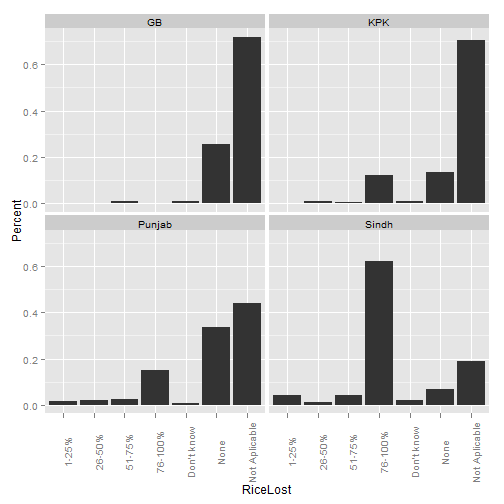
\includegraphics[width=.9\linewidth]{overall/figures/overallDistPlot} 

}


\end{knitrout}

\caption{Graphical view of the distribution of responses for all the data.\label{fig:fullDist}}
\end{figure}

In Section~\ref{sec:smallerDist} we analyze the distribution of responses for samples of fewer Tehsils.
